\documentclass{standalone}
\usepackage{tikz}

\begin{document}
    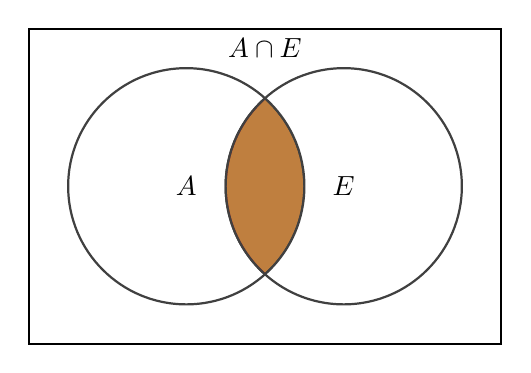
\begin{tikzpicture}[scale=1.0]
    	\def\circleA{(0,0) circle (1.5)} %A
    	\def\circleB{(0:2) circle (1.5)} %B
    
    	\colorlet{circle edgeA}{black!75} 
    	\colorlet{circle areaA}{red!100}
    	\colorlet{circle edgeB}{black!75} 
    	\colorlet{circle areaB}{green!100}
    
    	\tikzset{
    		filledA/.style={fill=circle areaA, draw=circle edgeA, thick},
    		filledB/.style={fill=circle areaB, draw=circle edgeB, thick},
    		outlineA/.style={draw=circle edgeA, thick},
    		outlineB/.style={draw=circle edgeB, thick},
    	}
    
    	\begin{scope}[fill opacity=0.5]         
    % 			\fill[filledB] \circleB;    
    % 			\fill[filledA] \circleA;
    			\clip \circleA;     
			        \fill[filledB] \circleB;
		        \clip \circleB;     
			        \fill[filledA] \circleA;
    	\end{scope}
    
    	\draw[outlineA] \circleA node {$A$}; 
    	\draw[outlineB] \circleB node {$E$}; 
    	\node[anchor=south] at (current bounding box.north) {$A \cap E$}; 
    	\draw[thick] (-2,-2) rectangle (4,2) node[anchor=south east] at (current bounding box.south east) { }; %U 
    \end{tikzpicture} 
\end{document}